\section{End-to-End Transfers}\label{sec:Transfers}
All of the transfers analyzed in this investigation arrive into the same Sun-Mars northern halo
orbit ($JC=3.0001857$) via the smallest periapsis stable manifold arc as the MMAT example in
\cref{fig:MMATSM}. However, the departure orbit in the Earth-Moon system varies, as well as the
unstable manifold arc departing the orbit. The arc selected depends on the category of transfer
being employed, and the end-to-end methodology for constructing both categories of transfers is as
follows:

\subsection{Transfers with Direct System Departure}
"Direct" transfers depart from the system directly along an Earth-Moon unstable invariant manifold
arc instead of utilizing a staging orbit, not to be confused with direct patched conic transfers
between the Earth and Mars.
\begin{enumerate}
    \item   Starting from the Earth-Moon CR3BP departure orbit, both unstable half-manifolds are
            propagated to the edge of the Earth SoI (ignoring those that crash into the Earth or
            Moon), where they are transformed into heliocentric Ecliptic J2000 states and
            propagated under Keplerian dynamics. The step is repeated for several different epochs
            during January 2026.
    \item   Each of the feasible manifold arcs then serves as a departure CR3BP arc and departure
            conic arc for the MMAT methodology introduced in \cref{sec:MMAT}. If they meet the MMAT
            inequality constraint (\cref{eq:MMAT}), then they produce two end-to-end direct
            transfers between an Earth-Moon and Sun-Mars orbit.
\end{enumerate}
An example direct transfer appears in \cref{fig:directE} and \cref{fig:directMMAT}. The departure
CR3BP arc originates from an Earth-Moon northern $L_{2}$ halo with a Jacobi constant of
$3.13$ in \cref{fig:directE}(a), appearing in the Earth-Moon rotating frame, and continues under
the Sun-Earth dynamics until it reaches the Earth SoI in \cref{fig:directE}(b). Note that the
trajectory is not optimized, nor is it the minimum-TOF or minimum-$\Delta v$ solution in the MMAT
family originating from that Earth-Moon departure orbit. This particular direct transfer has a
total maneuver cost of $5.544$ km/s with a total time-of-flight of $3.26$ years. The example direct
transfer highlights the potential of the transfer type, demonstrating the viability of employing
Earth-Moon unstable manifold arcs for efficient interplanetary transfers.

\begin{figure}[H]
    \begin{subfigure}[h]{0.495\linewidth}
        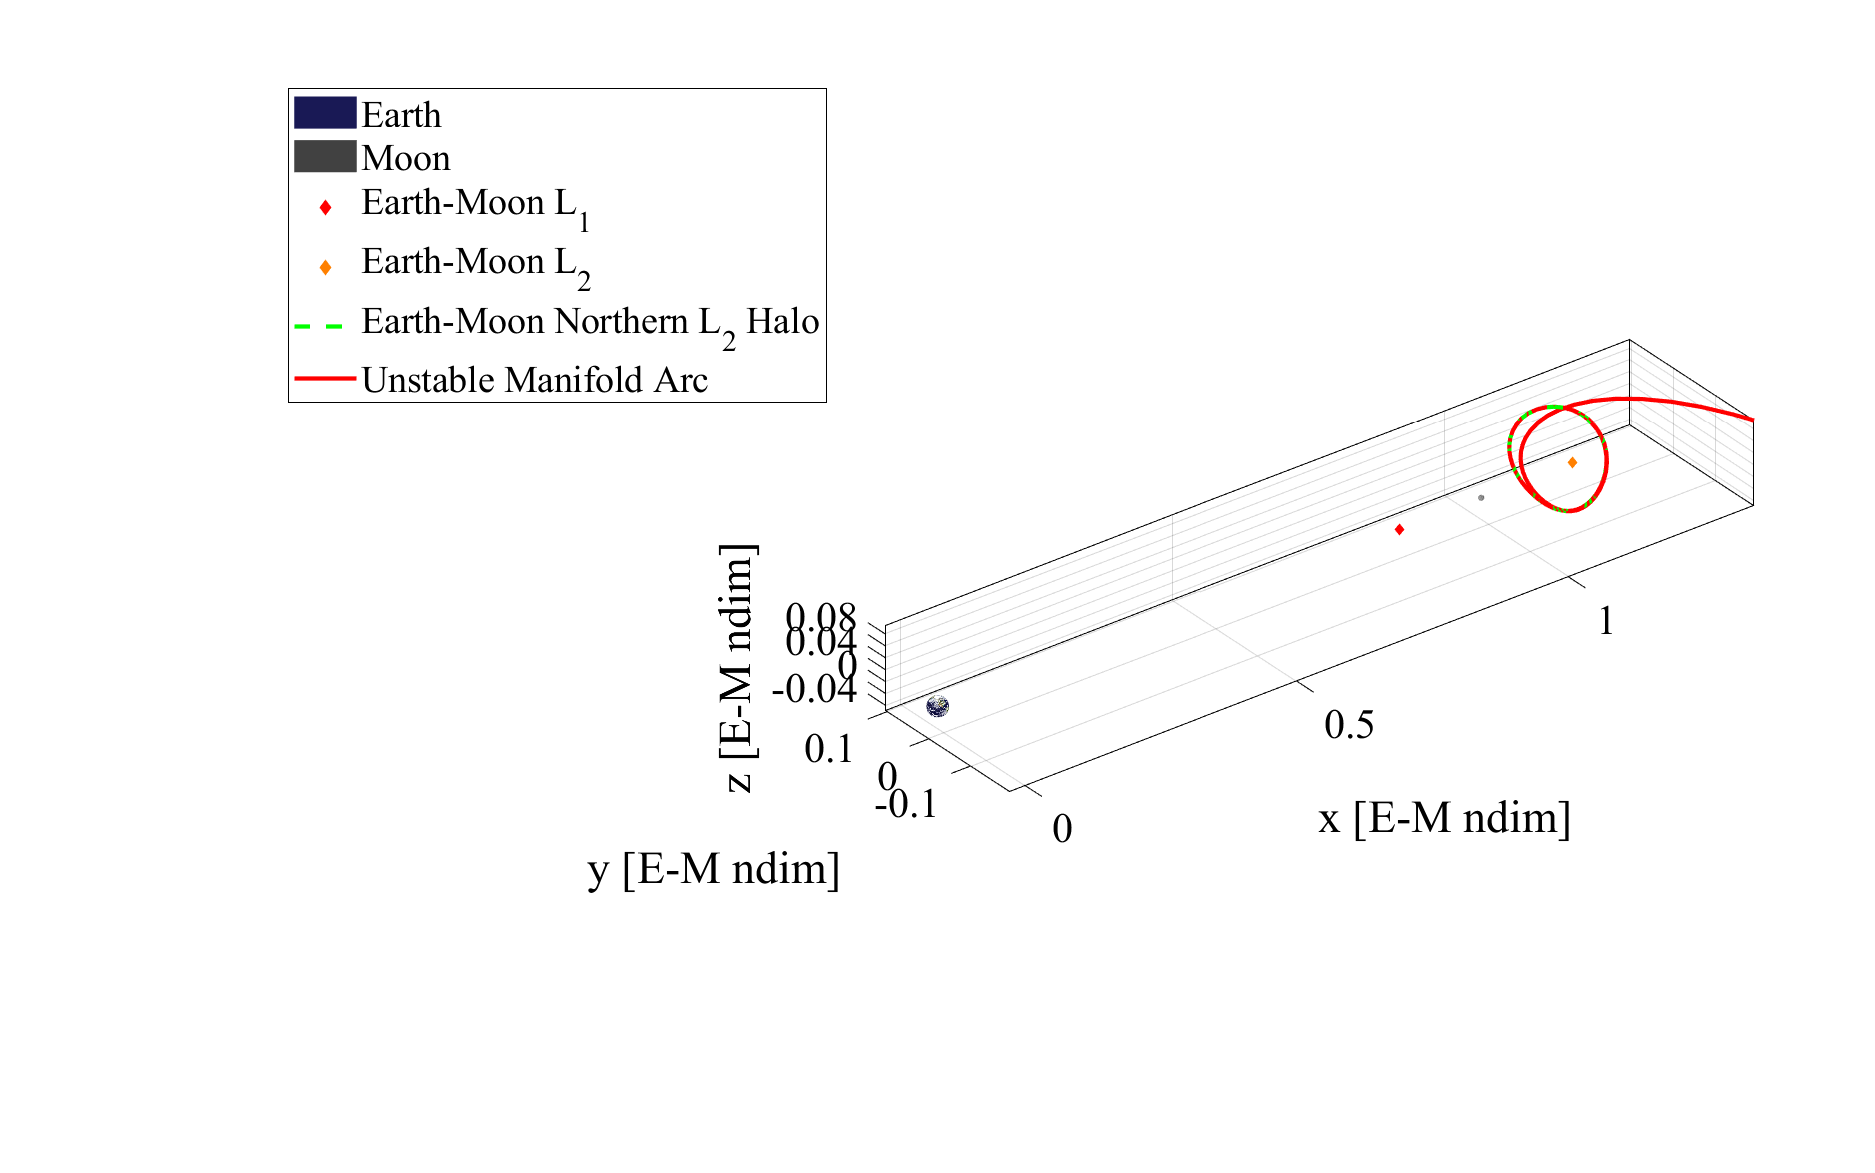
\includegraphics[width=\textwidth]{figures/DirectEM.pdf}
        \caption{Earth-Moon barycentric rotating frame.}
    \end{subfigure}
    \hfill
    \begin{subfigure}[h]{0.495\linewidth}
        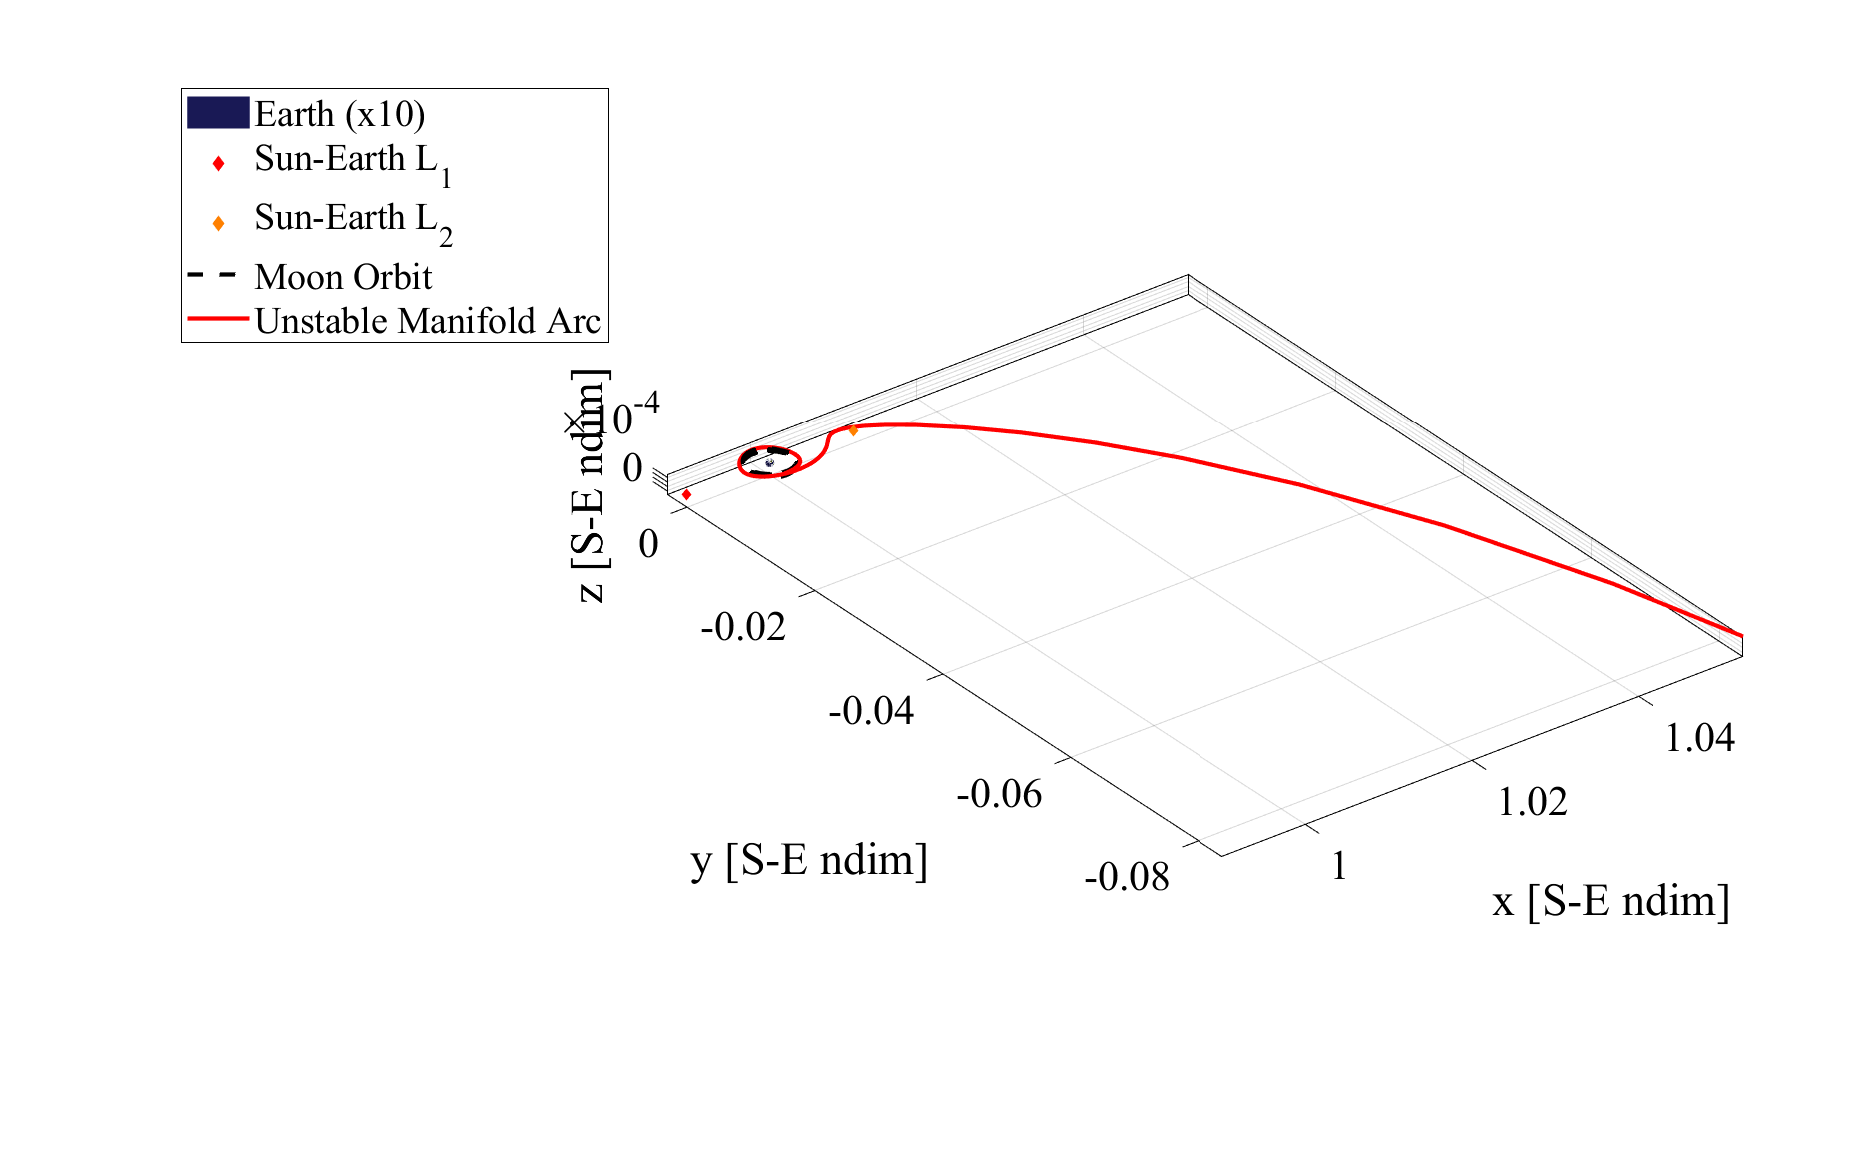
\includegraphics[width=\textwidth]{figures/DirectSE.pdf}
        \caption{Sun-Earth barycentric rotating frame.}
    \end{subfigure}
    \caption{Direct departure CR3BP arc.}
    \label{fig:directE}
\end{figure}

\begin{figure}[H]
    \centering
    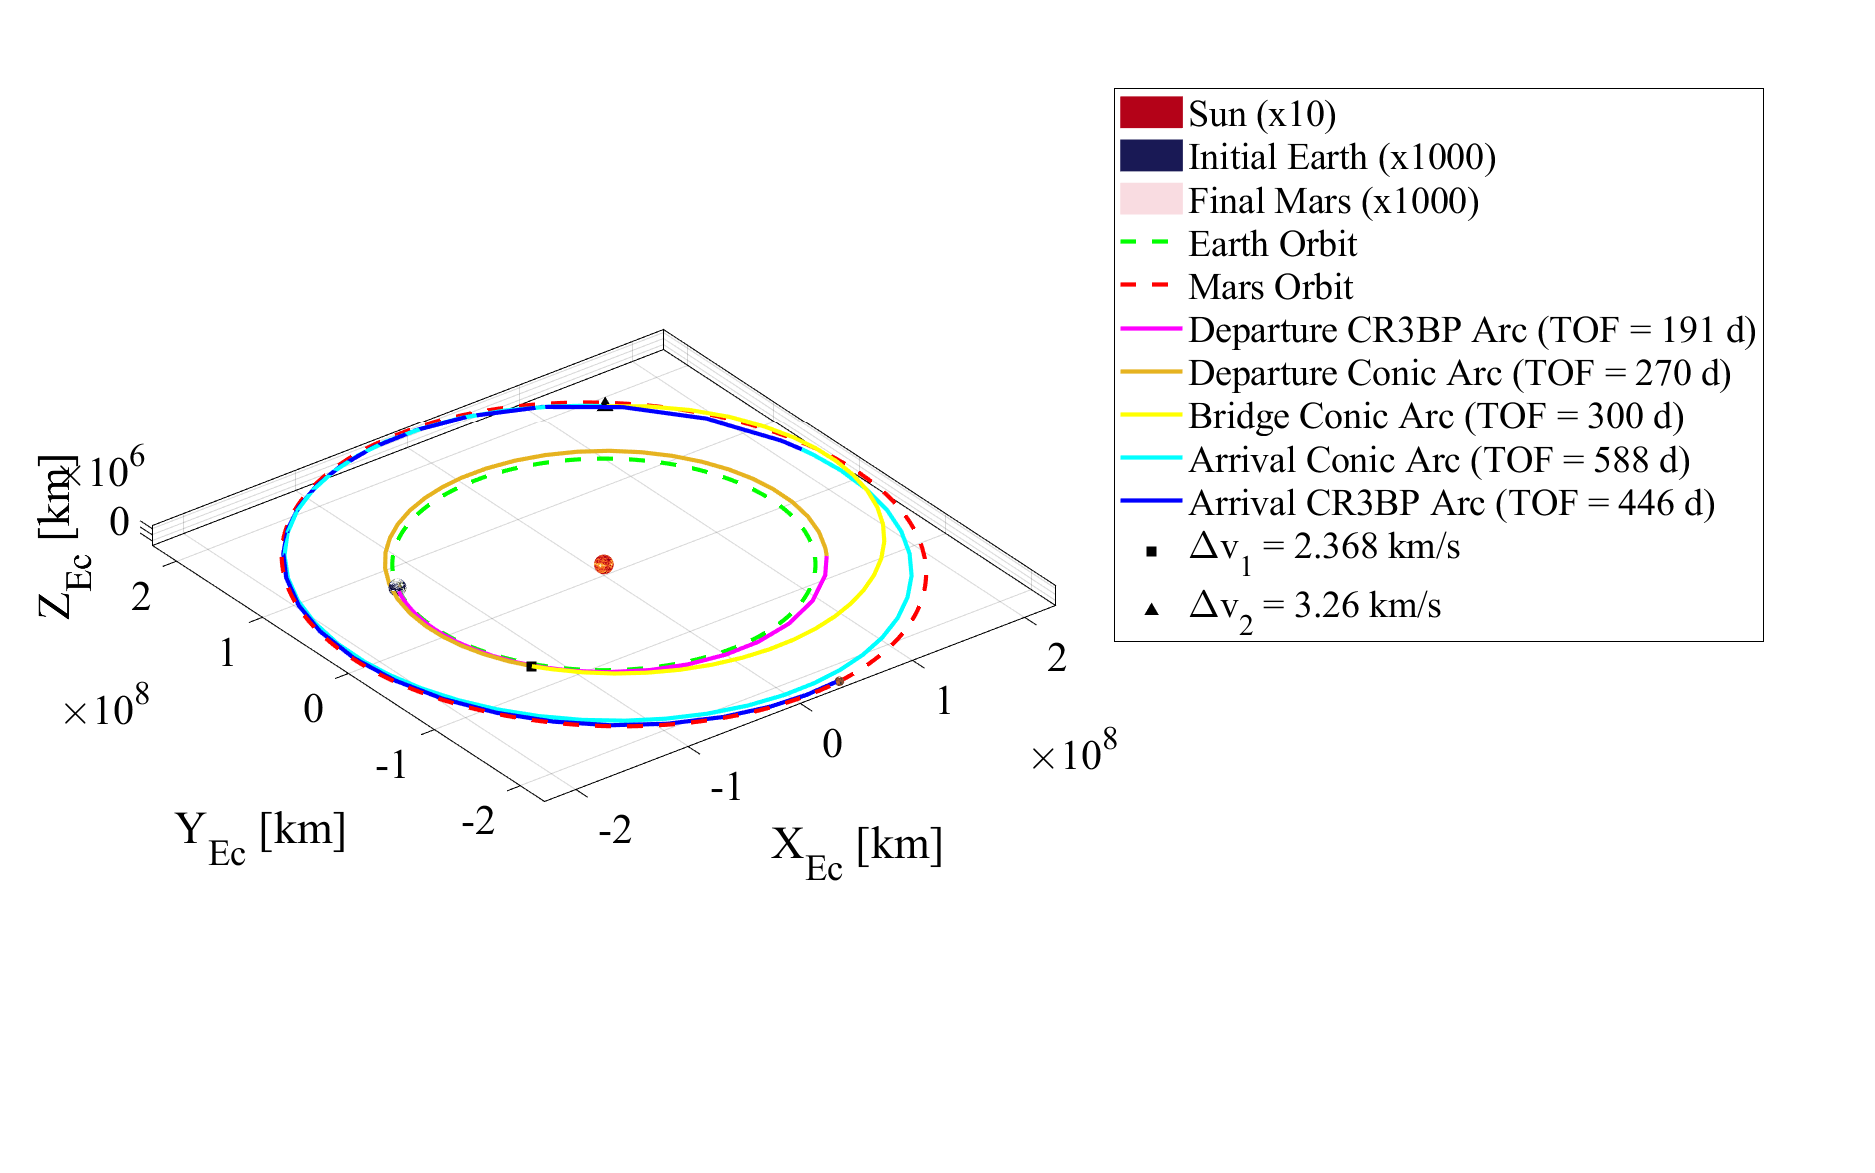
\includegraphics[width=0.9\textwidth]{figures/DirectMMAT.pdf}
    \caption{"Direct" MMAT in the Sun-centered Ecliptic J2000 frame.}
    \label{fig:directMMAT}
\end{figure}

\subsection{Transfers with an Intermediate Staging Orbit}
The staging orbit transfers connect Earth-Moon unstable invariant manifold arcs to Sun-Earth stable
manifold arcs before staging in a Sun-Earth $L_{2}$ northern halo orbit. After utilizing the orbit
to properly phase, the transfers depart from the system along a Sun-Earth unstable invariant
manifold arc.
\begin{enumerate}
    \item   Starting from the Earth-Moon CR3BP departure orbit, a near-ballistic transfer to a
            Sun-Earth CR3BP northern halo orbit is computed via the methodology introduced in
            \cref{sec:NearBallistic}. The particular Sun-Earth halo orbit is free to change to
            decrease the $\Delta v$ of the maneuver. The Earth-Moon to Sun-Earth portion of the
            trajectory dictates the initial epoch for the whole transfer.
    \item   Once in the Sun-Earth staging orbit, since the phase along the orbit is determined by
            the spacecraft arrival onto the orbit, unstable manifold arcs of the Sun-Earth halo
            orbit are propagated to the edge of the Earth SoI according to the time-correspondent
            location along the orbit. Each departure CR3BP manifold arc is then associated with a
            departure epoch from the Sun-Earth halo orbit.
    \item   Now, similar to the direct transfers, the arcs serve as the departure CR3BP arc and
            eventually the departure conic arc for the MMAT methodology (\cref{sec:MMAT}),
            producing two end-to-end transfers between the Earth-Moon and Sun-Mars orbits with an
            intermediate staging Sun-Earth halo orbit for each feasible manifold arc.
\end{enumerate}
\cref{fig:stagedEM}-\cref{fig:stagedMMAT} provide a sample transfer employing an intermediate
Sun-Earth staging halo orbit. The departure from the Earth-Moon orbit in \cref{fig:stagedEM} is
similar to the direct transfer example, utilizing the same $L_{2}$ halo orbit. However, a different
manifold arc is employed for this transfer. The near-ballistic transfer appears in
\cref{fig:stagedSE}, where the Earth-Moon orbit is connected to the Sun-Earth northern halo staging
orbit. The departure CR3BP arc is also provided leaving the staging orbit along the unstable
manifold, that is then employed in the MMAT in \cref{fig:stagedMMAT}. Once again, the solution is
not optimized, with a total maneuver cost of $5.481$ km/s and a time-of-flight of $4.59$ years. The
example staging orbit trajectory highlights the potential application of the transfer type,
demonstrating the viability of Sun-Earth intermediate orbits to properly phase interplanetary
transfers.

\begin{figure}[H]
    \centering
    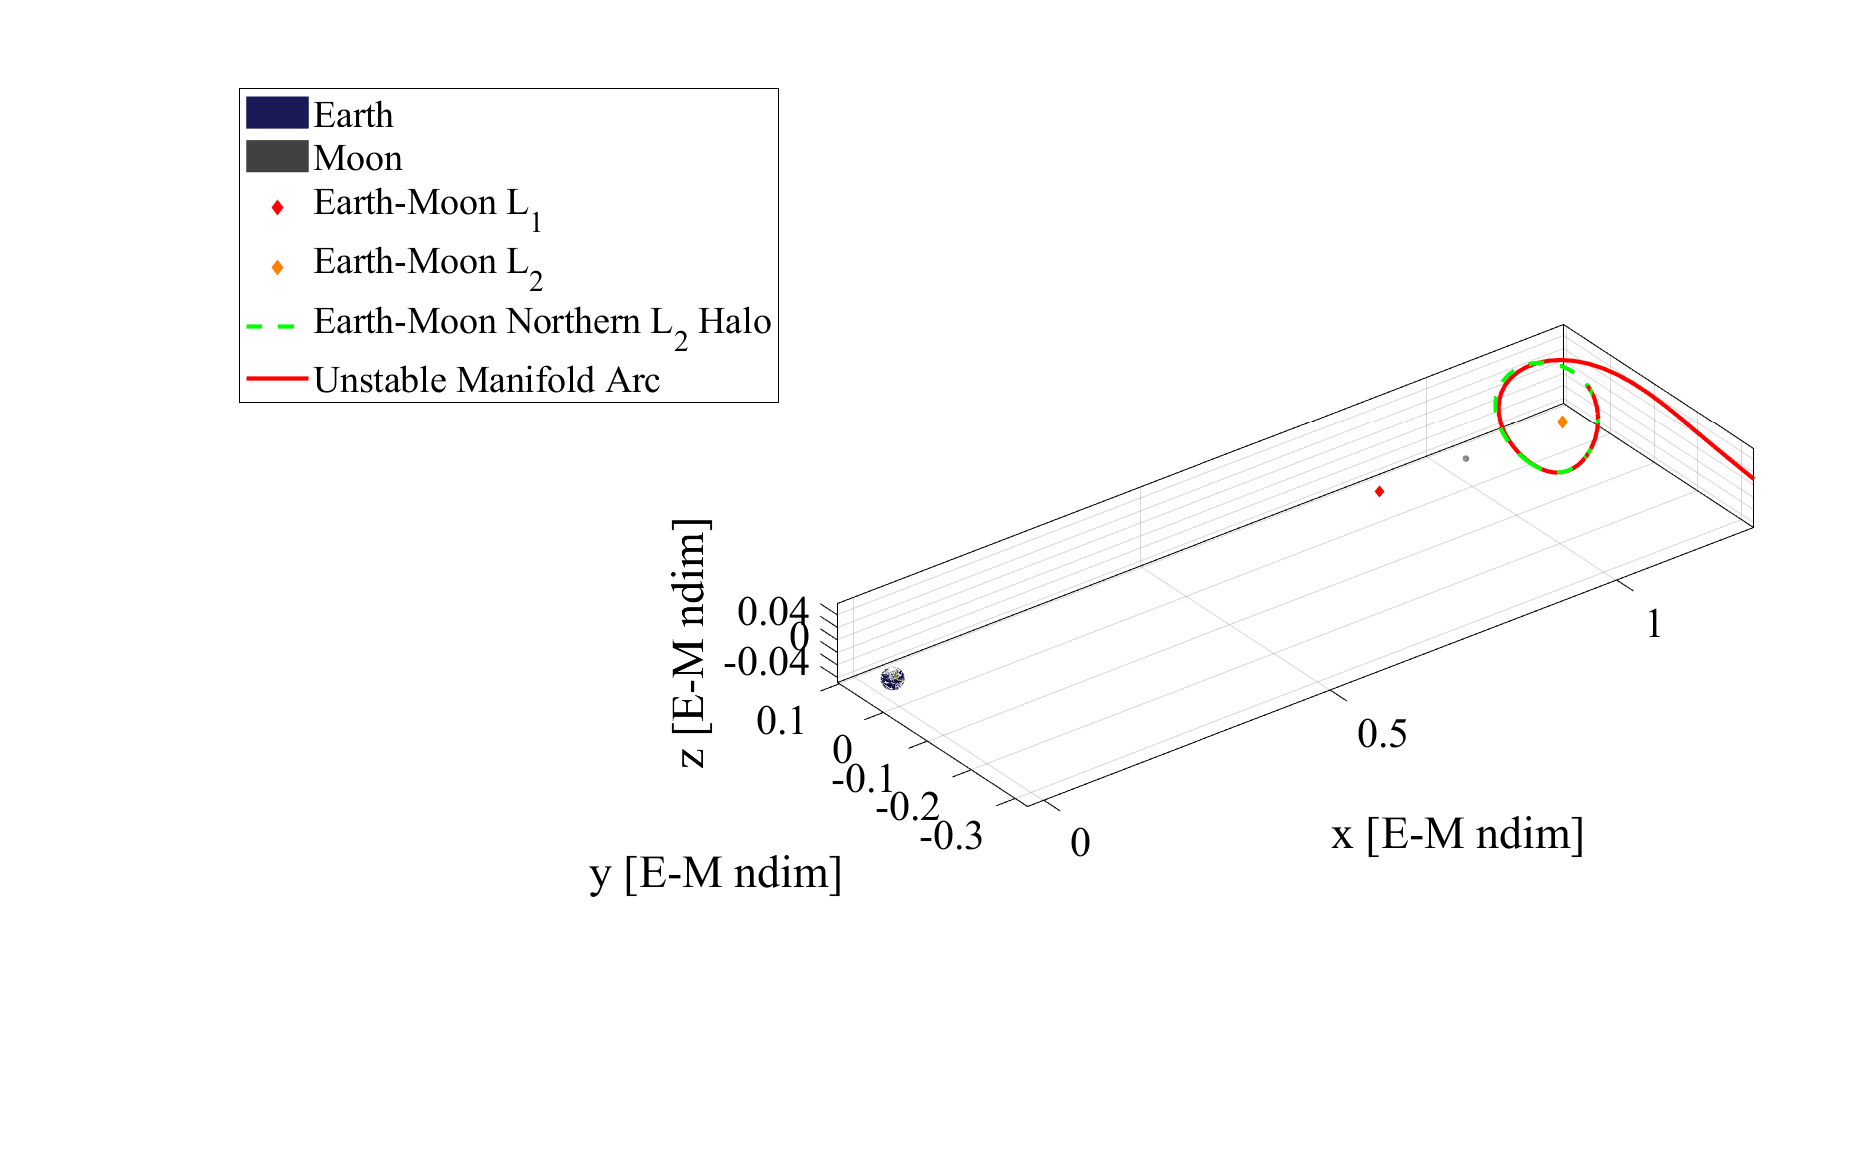
\includegraphics[width=0.9\textwidth]{figures/StagedEM.pdf}
    \caption{Departure unstable manifold arc in the Earth-Moon barycentric rotating frame.}
    \label{fig:stagedEM}
\end{figure}

\subsection{Transfer Tradespace}
As mentioned, both categories of transfers exist in families, so the available solutions have a
range of total maneuver $\Delta v$ costs and times-of-flight. \cref{fig:tradespace} provides one
such tradespace for transfers originating from a $JC=3.13$ Earth-Moon northern $L_{2}$ halo orbit
(the same employed in the previous examples). In the figure, the red points represent the family of
transfers that include a staging orbit, while the blue points represent the family of direct
transfers. The black modified Hohmann transfer line serves as a $\Delta v$ baseline for comparison.
The tradespaces provide valuable insight into the performance of the two transfer strategies,
enabling mission designers to balance maneuver costs and time-of-flight against mission
requirements and constraints.

\begin{figure}[H]
    \centering
    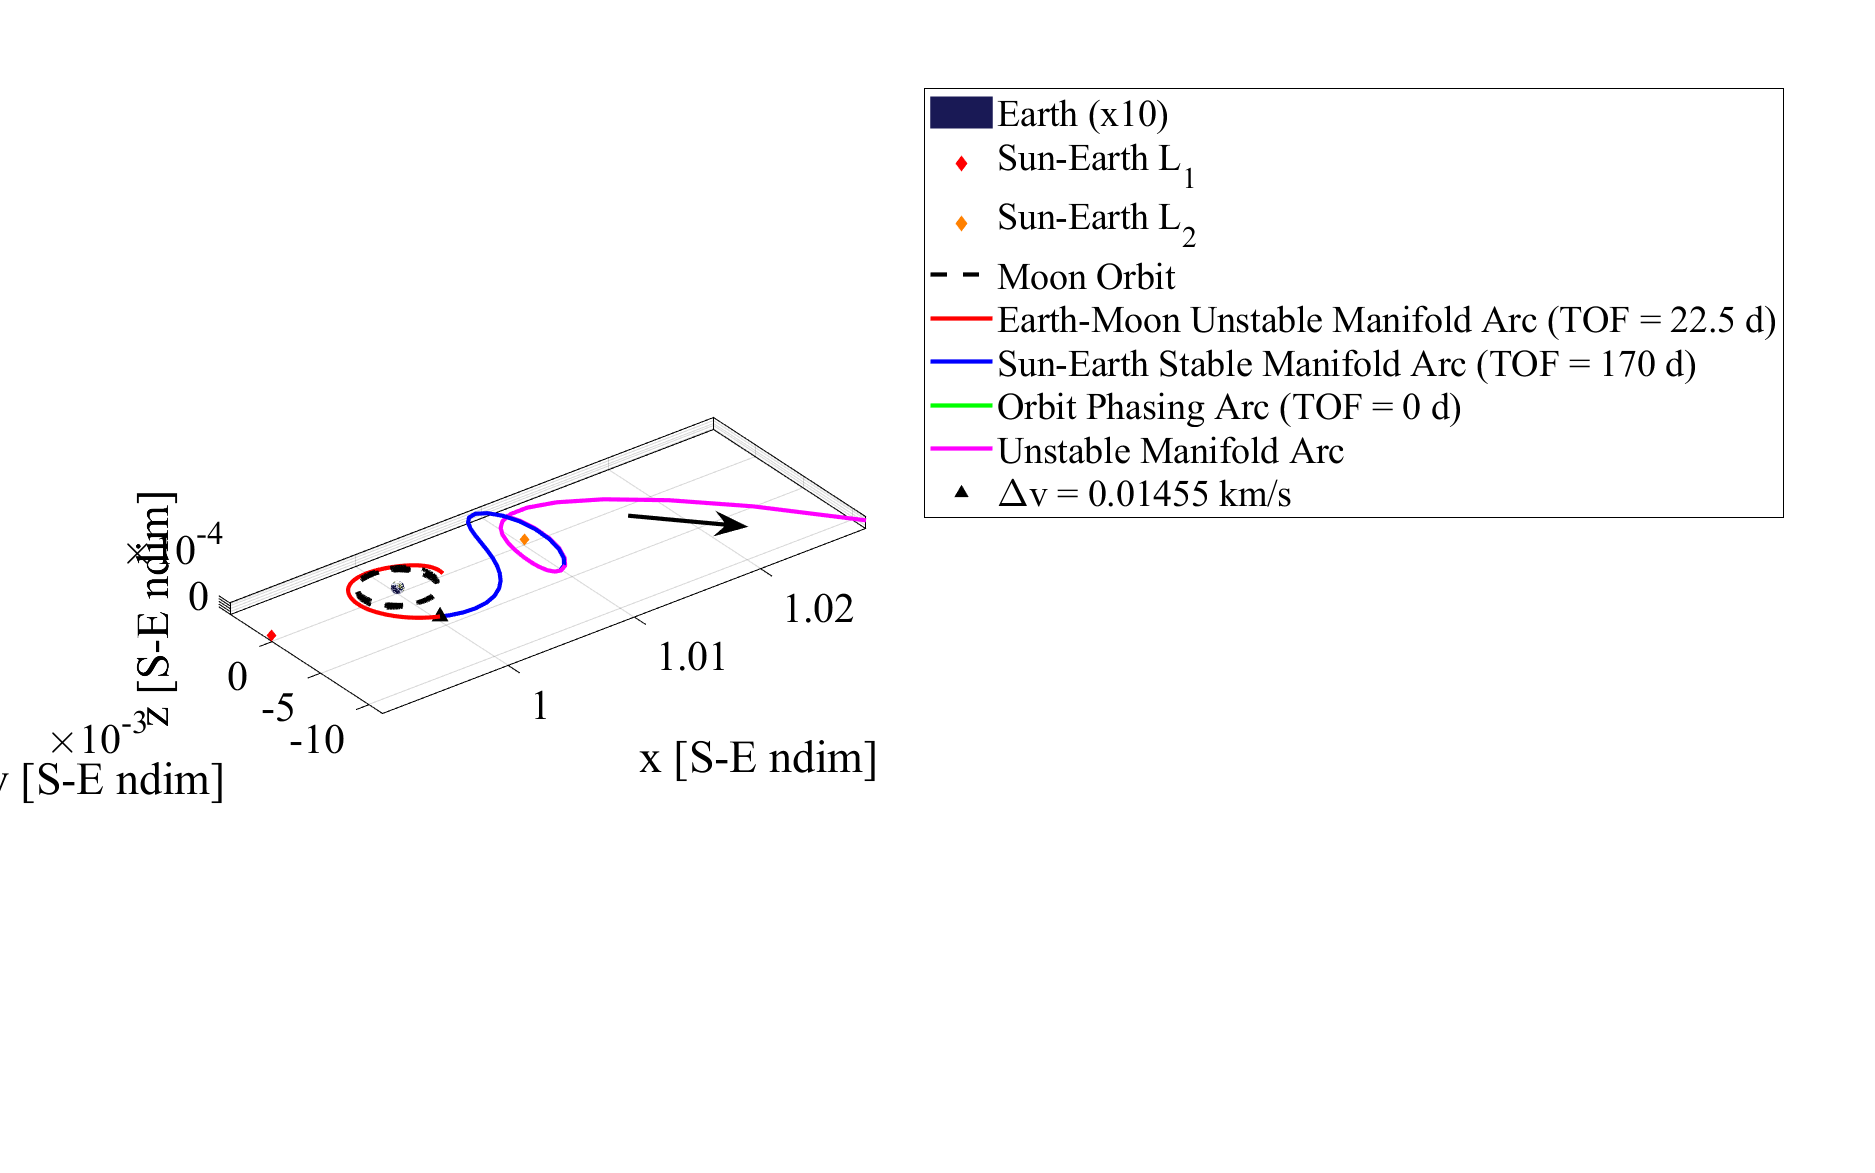
\includegraphics[width=0.9\textwidth]{figures/StagedSE.pdf}
    \caption{Departure CR3BP arc with staging orbit in the Sun-Earth barycentric rotating frame.}
    \label{fig:stagedSE}
\end{figure}

\begin{figure}[H]
    \centering
    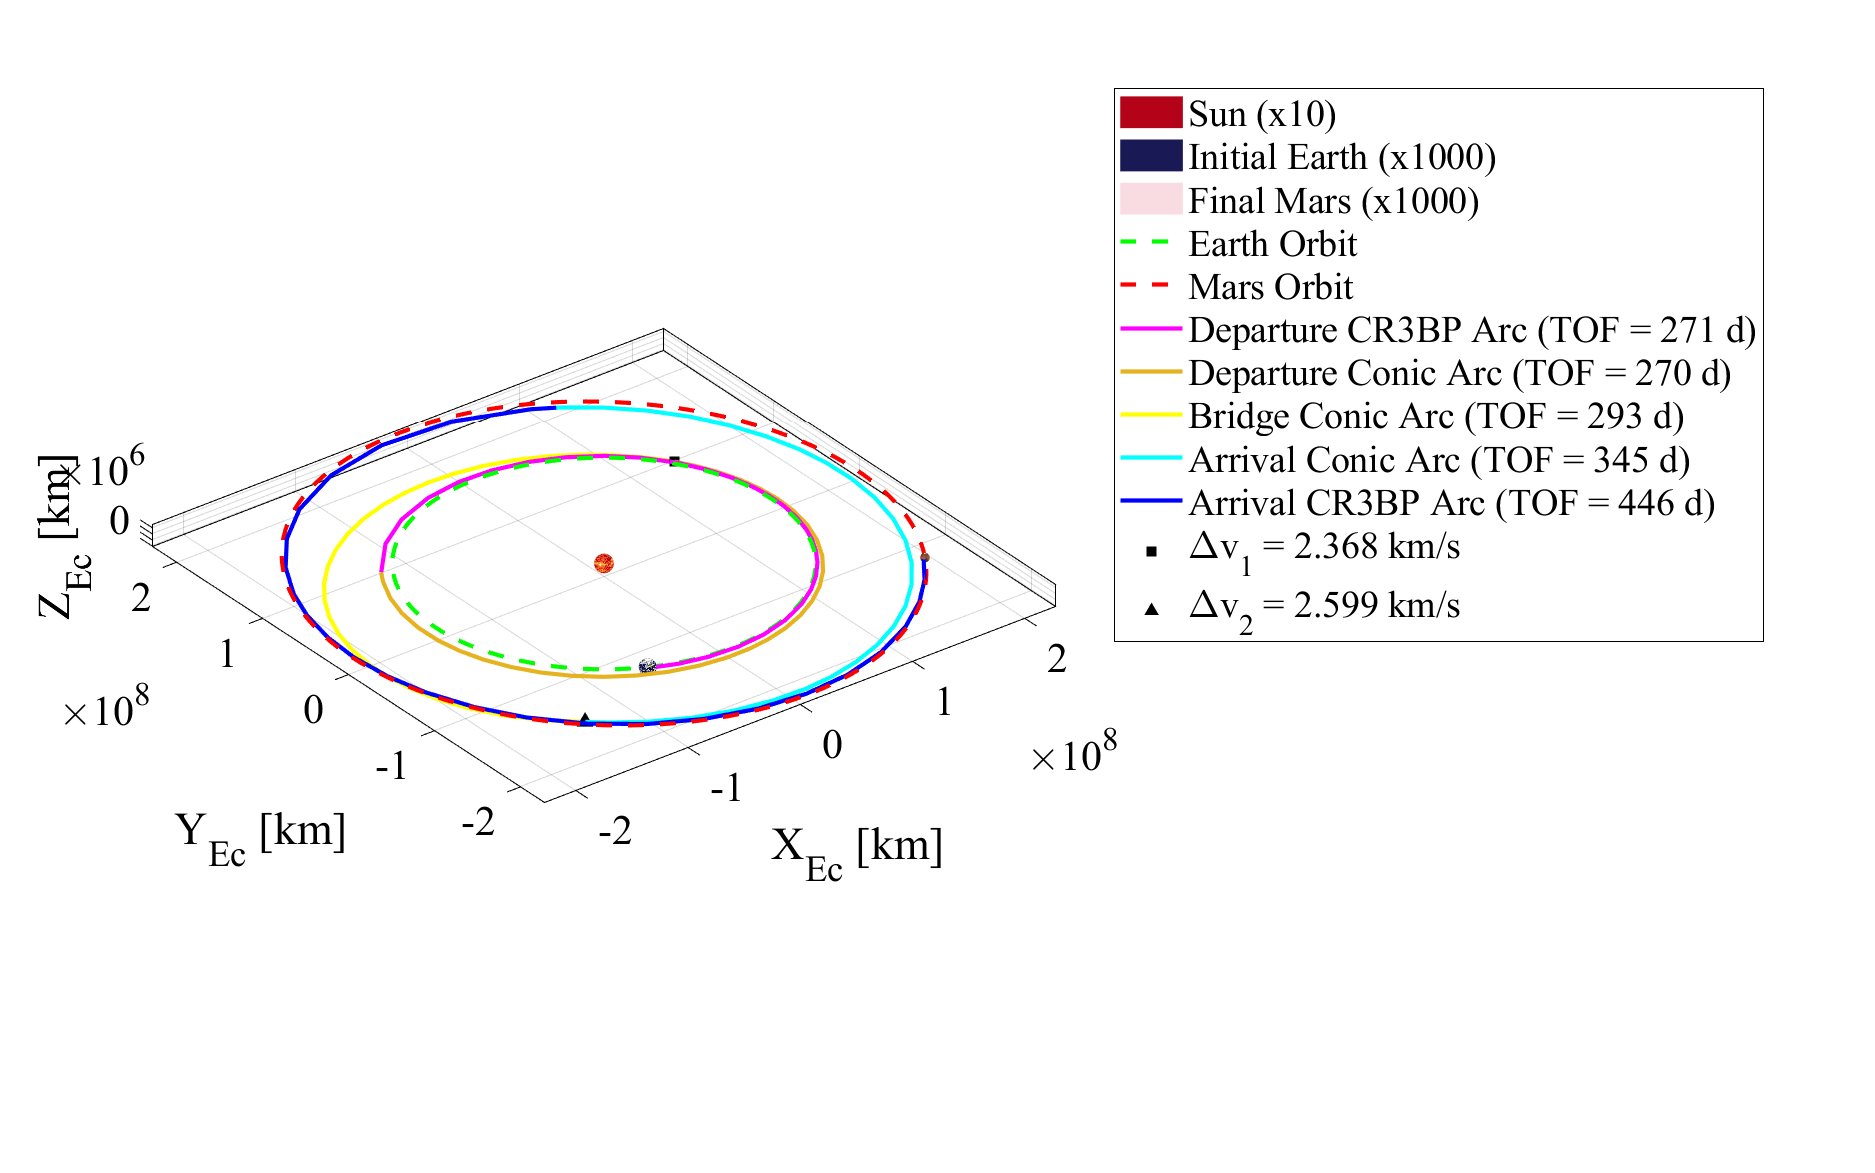
\includegraphics[width=0.9\textwidth]{figures/StagedMMAT.pdf}
    \caption{MMAT with staging orbit in the Sun-centered Ecliptic J2000 frame.}
    \label{fig:stagedMMAT}
\end{figure}

\begin{figure}[ht]
    \centering
    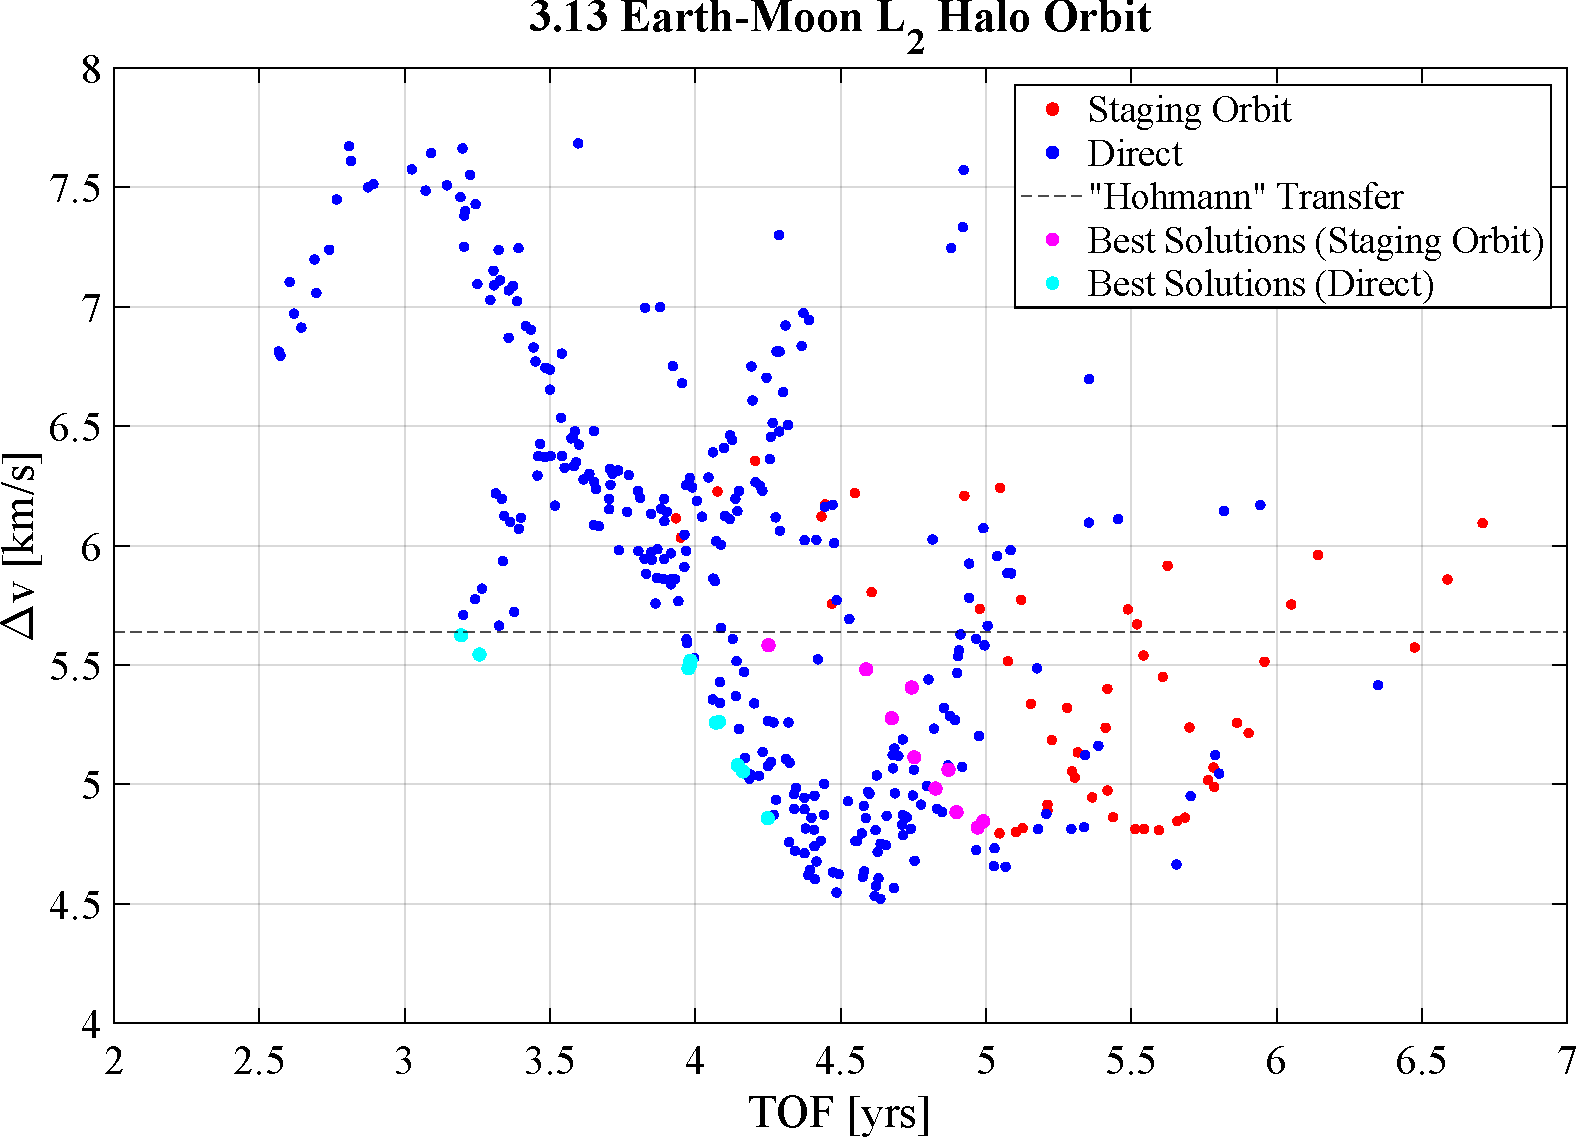
\includegraphics[width=0.75\textwidth]{figures/TradeSpace_L2Halo_3_13.pdf}
    \caption{Tradespace of both solution categories originating from the same Earth-Moon departure orbit.}
    \label{fig:tradespace}
\end{figure}
